\documentclass[aps,prx]{revtex4-2}

\usepackage{graphicx}

\usepackage{dcolumn}% Align table columns on decimal point
\usepackage{bm}% bold math
%\usepackage[mathlines]{lineno}% Enable numbering of text and display math
%\linenumbers\relax % Commence numbering lines

\usepackage[utf8]{inputenc}
\usepackage[T1]{fontenc}
\usepackage{mathptmx}
\usepackage{etoolbox}
\usepackage{siunitx}
\usepackage{amsmath}
\usepackage{float}

\usepackage{physics}

\renewcommand{\thefigure}{S\arabic{figure}}
\renewcommand{\thetable}{S\arabic{table}}
\renewcommand{\theequation}{S\arabic{equation}}
\usepackage{xcolor}

\newenvironment{myfont}{\fontfamily{ptm}\selectfont}{\par}
\DeclareTextFontCommand{\textmyfont}{\myfont}

\newcommand{\AI}[1]{\textcolor{black}{#1}} 

\makeatletter
\def\@email#1#2{%
 \endgroup
 \patchcmd{\titleblock@produce}
  {\frontmatter@RRAPformat}
  {\frontmatter@RRAPformat{\fontsize{9}{10}\selectfont\produce@RRAP{ Authors to whom the correspondence should be addressed: {#2}}}\frontmatter@RRAPformat}
  {}{}
}%
\makeatother

\begin{document}
\onecolumngrid

\title{Supplementary Material: Sometimes on EO qubits} 

\author{TV or DC}
\thanks{These authors contributed equally}
\affiliation{QuTech and Kavli Institute of Nanoscience, Delft University of Technology, PO Box 5046, 2600 GA Delft, The Netherlands}
\author{TV or DC}
\thanks{These authors contributed equally}
\affiliation{QuTech and Kavli Institute of Nanoscience, Delft University of Technology, PO Box 5046, 2600 GA Delft, The Netherlands}
\author{Valentin John}
\affiliation{QuTech and Kavli Institute of Nanoscience, Delft University of Technology, PO Box 5046, 2600 GA Delft, The Netherlands}
\author{Cecile X. Yu}
\affiliation{QuTech and Kavli Institute of Nanoscience, Delft University of Technology, PO Box 5046, 2600 GA Delft, The Netherlands}
\author{Francesco Borsoi}
\affiliation{QuTech and Kavli Institute of Nanoscience, Delft University of Technology, PO Box 5046, 2600 GA Delft, The Netherlands}
\author{Stefan D. Oosterhout}
\affiliation{QuTech and Netherlands Organisation for Applied Scientific Research (TNO), Delft, The Netherlands}
\author{Lucas E. Stehouwer}
\affiliation{QuTech and Kavli Institute of Nanoscience, Delft University of Technology, PO Box 5046, 2600 GA Delft, The Netherlands}
\author{Giordano Scappucci}
\affiliation{QuTech and Kavli Institute of Nanoscience, Delft University of Technology, PO Box 5046, 2600 GA Delft, The Netherlands}
\author{Stefano Bosco}
\affiliation{QuTech and Kavli Institute of Nanoscience, Delft University of Technology, PO Box 5046, 2600 GA Delft, The Netherlands}
\author{Maximilian Rimbach-Russ}
\affiliation{QuTech and Kavli Institute of Nanoscience, Delft University of Technology, PO Box 5046, 2600 GA Delft, The Netherlands}
\author{Barnaby van Straaten}
\affiliation{QuTech and Kavli Institute of Nanoscience, Delft University of Technology, PO Box 5046, 2600 GA Delft, The Netherlands}
\author{Menno Veldhorst}
\affiliation{QuTech and Kavli Institute of Nanoscience, Delft University of Technology, PO Box 5046, 2600 GA Delft, The Netherlands}


\email{m.veldhorst@tudelft.nl, m.f.russ@tudelft.nl}

\maketitle
\newpage

\section{Basic characterization}

\begin{figure*}
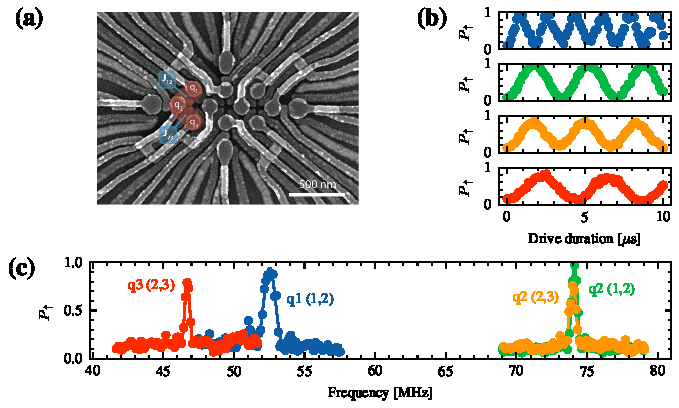
\includegraphics[width=\textwidth]{figures/supp1/main.pdf}
\caption{\textbf{Basic spin characterization.} \textbf{(a)} Device SEM. \textbf{(b)} single spin rabi driving. \textbf{(c)} EDSR resonances.}
\label{fig:edsr-spectrum}
\end{figure*}

\section{Some data/derivations}

\section{Some more data/derivations}

\bibliography{references}

\end{document}